% !TEX root = ./main.tex

Foundation models (FM) are a type of artificial intelligence (AI)
model designed for learning generic representations from data. They
typically employ unsupervised learning techniques and fall under the
umbrella of representation learning. This chapter includes an overview
of Vision Foundation Models (VFMs). Foundation Models, like all AI
models, have the following components: model architecture, dataset,
objective (training strategy), and optimizer.

\begin{itemize}
    \item \emph{Model architecture}: This is used to store the
        parameters and decides how operations are preformed on the
        input data. They are usually multi-layer perceptrons (MLPs),
        convolution \cite{LeCun1998GradientbasedLA}, and/or
        transformer \cite{Dosovitskiy2020AnII, Vaswani2017AttentionIA}
        layers. Recent developments include MLP mixer
        \cite{Tolstikhin2021MLPMixerAA}, ConvNext \cite{Liu2022ACF},
        and some transformer variants (Swin Transformer
        \cite{Liu2021SwinTV, Liu2021SwinTH}, CCT
        \cite{Hassani2021EscapingTB}, etc). 
    \item \emph{Dataset}: This is the source of learning for the FM.
        Usually, these are large datasets that contain samples from a
        wide distribution. Some common publicly available datasets in
        vision are ImageNet \cite{Deng2009ImageNetAL} and Tencent
        ML-Images \cite{Wu2019TencentMA}. Some proprietary datasets
        include JFT-300M \cite{Sun2017RevisitingUE}, JFT-3B
        \cite{Zhai2021ScalingVT} (Google), and IG-3.5B
        \cite{Mahajan2018ExploringTL} (Facebook/Meta).
    \item \emph{Objective, training strategy and loss function}: Since
        the datasets are non-labelled and manual annotation is
        difficult, the training strategy must include some form of
        self-supervision to facilitate representation learning. These
        include techniques like knowledge distillation
        \cite{Hinton2015DistillingTK}, masked representation learning
        \cite{He2021MaskedAA}, and various contrastive learning
        techniques and losses that aim to align modalities. Some
        implementations include MoCo \cite{He2019MomentumCF,
        Chen2020ImprovedBW}, SwAV \cite{Caron2020UnsupervisedLO},
        SimCLR \cite{Chen2020ASF, Chen2020BigSM}, BYOL
        \cite{Grill2020BootstrapYO}, etc.
    \item \emph{Optimizer}: These are used to tune the model's
        parameters. Usually, optimizers like the Adam
        \cite{Kingma2014AdamAM} and its recent development, AdamW
        \cite{Loshchilov2017DecoupledWD}, are well suited. However,
        since the number of parameters often run into hundreds of
        mullions (and often billions), it makes heavy use of
        parallelization techniques like data sharding and model
        splitting across GPUs. Common implementations of parallel
        optimizers include Fully Sharded Data Parallel (FSDP)
        \cite{Xu2020AutomaticCS} (part of FairScale and PyTorch), Zero
        Redundancy Optimizer (ZeRO) \cite{Wang2023ZeROEE,
        Rajbhandari2019ZeROMO}, DeepSpeed \cite{Li2022DeepSpeedDE},
        Megatron \cite{Narayanan2021EfficientLL}, etc.
\end{itemize}

This chapter gives an overview of model architectures and training
strategies involved in DINO \cite{Caron2021EmergingPI} and DINOv2
\cite{Oquab2023DINOv2LR}, which are the vision backbones used for this
work. A thorough review on self-supervised learning (SSL) and
foundation models can be found in \cite{Balestriero2023ACO,
Gui2023ASO, Jaiswal2020ASO}.

\section{Vision Transformers}

\subsection{ViT}
\label{subsec:vit}

Vision Transformers (ViTs) \cite{Dosovitskiy2020AnII} are inspired
from transformers in Natural Language Processing (NLP)
\cite{Vaswani2017AttentionIA}, which in turn are inspired by
\emph{information retrieval} using queries in a key-value database.
They operate in a manner described below (and shown in
\cref{fig:vit_input_patchification,fig:vit_encoder_mha})

\begin{figure}
    \centering
    \includegraphics[width=\textwidth]{vision_transformer_img_overview.pdf}
    \caption{Data processing for Vision Transformers}
    \small
        Input image is first broken into patches. These patches are
        flattened and a (shared) linear projection is applied to all
        of them. A $\left[CLS\right]$ token is added for global
        context. Then, position embeddings are added to each element
        and the entire set in concatenated into a vector (with the
        $\left[CLS\right]$ - denoted in blue squared - usually going
        first). The $\cdot$ (dot) signifies addition of position
        embeddings and $\oplus$ signifies concatenation. \\
        Image is best viewed in color.
    \label{fig:vit_input_patchification}
\end{figure}

\paragraph{Step 1 - Patchification of the Input Image}

As shown in \cref{fig:vit_input_patchification}, an input image
$\mathbf{I} \in \mathbb{R}^{C, H, W}$ is split into patches of shape
$s_h, s_w$ each, giving $n_h = H/s_h$ patches along height and $n_w =
W/s_w$ patches along width. These $n = n_h \times n_w$ patches are
then flattened into $d_m = C \times s_h \times s_w$ dimensional
vectors. Each patch is multiplied by a \emph{shared} square linear
matrix, keeping the output dimensionality same. We obtain the
transformed patch embeddings as $\left\{ \mathbf{p}_i \in
\mathbb{R}^{d_m} \right\}_{i = [1, n]}$. For utilizing global context,
a learnable $\mathbf{p}_0 = \left[CLS\right]$ token (same shape as the
patch vectors) is added to the set. These $n+1$ patches are then
transformed by adding position embeddings (so that each element in the
sequence gets a notion of its position in the sequence). Finally,
they're all concatenated into a vector. The final input to the model
is given by the vector $\mathbf{x} \in \mathbb{R}^{(1+n) \times d_m}$
(with the first $d_m$ values for the $\left[CLS\right]$ token). This
vector $\mathbf{x}$ is the input to the transformer layers. For
simplicity, we use $l = 1 + n$ for sequence length hereon.

\begin{figure}
    \centering
    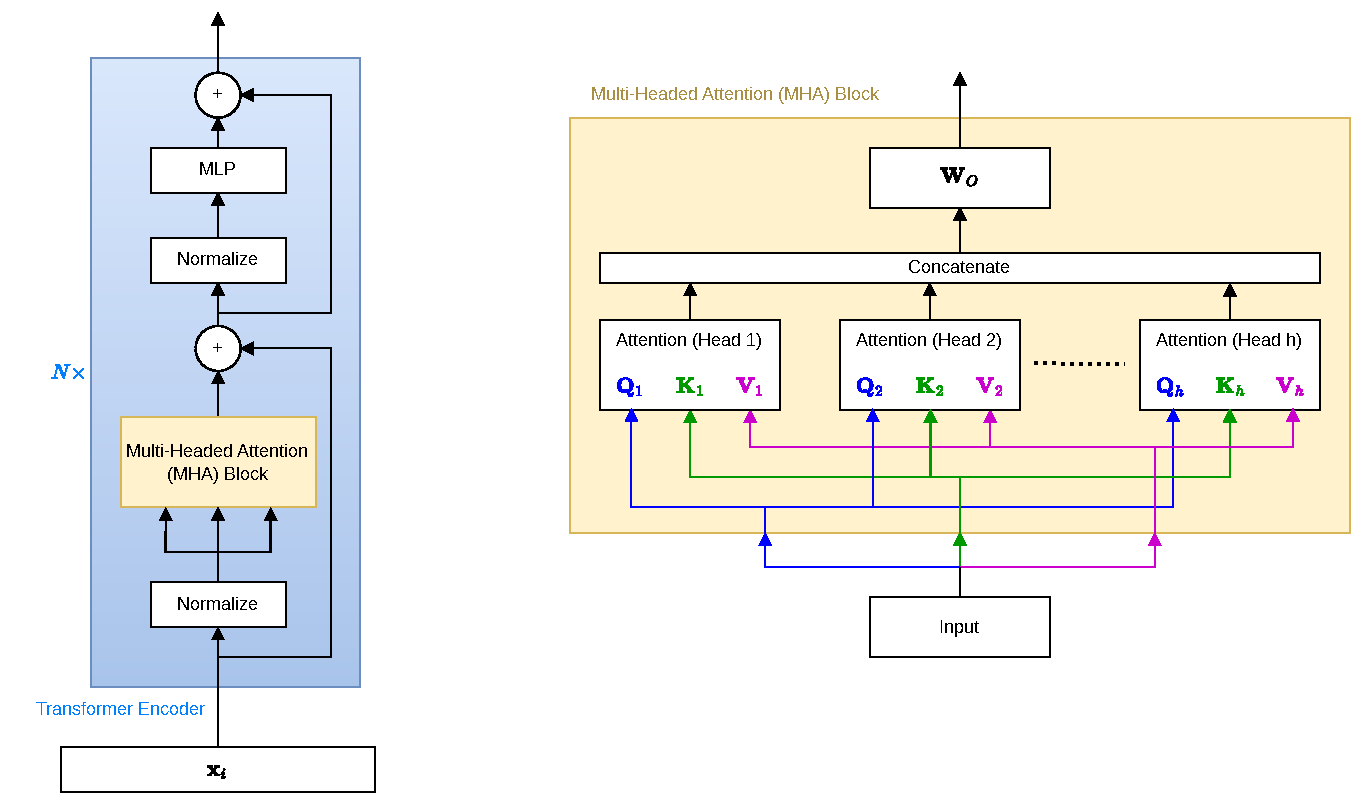
\includegraphics[width=\textwidth]{vision_transformer_encoder_mha.pdf}
    \caption{Transformer Encoder and Multi-Headed Attention}
    \small
        Each transformer encoder block contains multi-headed attention
        block. The $+$ operations denote addition of residuals. Each
        head has its own query $\mathbf{Q}_i$, key $\mathbf{K}_i$ and
        value $\mathbf{V}_i$ vectors and applies self-attention. \\
        Image is best viewed in color.
    \label{fig:vit_encoder_mha}
\end{figure}

\paragraph{Step 2 - Transformer Encoders with Multi-headed Attention}

As shown in figure \cref{fig:vit_encoder_mha}, the input is given to
$N$ transformer encoder blocks, which are linked in sequence. Each
block normalizes its input, passes it through a multi-headed attention
(MHA) layer in residual, it finally passes it through an MLP block in
the same normalization and residual manner. LayerNorm
\cite{Ba2016LayerN} is used instead of BatchNorm
\cite{Ioffe2015BatchNA} because it is easier to parallelize and can
deal with varying batch sizes. Each head (say head $i$) of MSA does
the following

\begin{enumerate}
    \item The input $\mathbf{x} \in \mathbb{R}^{l, d_m}$ (where $l =
        1+n$ is the sequence length and $d_m$ is the feature
        dimension) is passed through LayerNorm, giving
        $\tilde{\mathbf{x}} = \mathrm{LN}(\mathbf{x})$ (where
        $\tilde{\mathbf{x}} \in \mathbb{R}^{l, d_m}$). We then apply
        weights $\mathbf{W}_{Qi} \in \mathbb{R}^{d_m, d_k}$ for query,
        $\mathbf{W}_{Ki} \in \mathbb{R}^{d_m, d_k}$ for key, and
        $\mathbf{W}_{Vi} \in \mathbb{R}^{d_m, d_k}$ for value. Here,
        $d_k = d_m / h$, where $h$ is the number of heads ($h$ is
        chosen such that it divides $d_m$). We get the query
        $\mathbf{Q}_i \in \mathbb{R}^{l, d_k}$, key $\mathbf{K}_i \in
        \mathbb{R}^{l, d_k}$, and value $\mathbf{V}_i \in
        \mathbb{R}^{l, d_k}$ vectors using
        \begin{align}
            \mathbf{Q}_i &= \tilde{\mathbf{x}} \mathbf{W}_{Qi} &
            \mathbf{K}_i &= \tilde{\mathbf{x}} \mathbf{W}_{Ki} &
            \mathbf{V}_i &= \tilde{\mathbf{x}} \mathbf{W}_{Vi}
        \end{align}
    
    \item The output of the self-attention $\mathbf{A}_{i} \in
        \mathbb{R}^{l, d_k}$ is given
        by
        \begin{align}
            \mathbf{A}_i = \mathrm{Attention}(\mathbf{Q}_i, 
                \mathbf{K}_i, \mathbf{V}_i) = \mathrm{softmax} \left(
                    \frac{\mathbf{Q}_i \mathbf{K}_i^\textup{T}}
                        {\sqrt{d_k}}\right) \mathbf{V}_i
        \end{align}
        The above equation is similar to information retrieval where a
        query is matched with key using $d_k$ dimensional embeddings
        to retrieve value (information). This formulates it in a
        differentiable and continuous manner. The $\mathrm{softmax}$
        uses $\sqrt{d_k}$ for normalization and does row-wise
        normalization.
    
    \item The output across all heads is concatenated (along the $d_k$
        dimension of each vector) into a single vector $\mathbf{A} \in
        \mathbb{R}^{l, d_m}$ using
        \begin{equation}
            \mathbf{A} = \left[\mathbf{A}_1 \oplus \mathbf{A}_2 \oplus 
                \cdots \oplus \mathbf{A}_i \oplus \cdots \mathbf{A}_h
                \right]
        \end{equation}
    
    \item The final output $\mathbf{y} \in \mathbb{R}^{l, d_m}$ of the
        MHA block is given by applying a linear transformation through
        weights $\mathbf{W}_O \in \mathbb{R}^{d_m, d_m}$, given by
        \begin{equation}
            \mathbf{y} = \mathbf{A} \mathbf{W}_O
        \end{equation}
        The weights $\mathbf{W}_O$ mix the outputs across all heads.
\end{enumerate}

\paragraph{Step 3 - Normalize and Linear Transform}

The output of MHA block $\mathbf{y} \in \mathbb{R}^{l, d_m}$ is then
added with the input $\mathbf{x} \in \mathbb{R}^{l, d_m}$ (residual
connection). The result is then passed through LayerNorm
\cite{Ba2016LayerN} (along the $d_m$ dimension) and then a 2-layer MLP
where first layer expands the dimension from $d_m$ to $4d_m$, and the
second layer reduces the dimension form $4d_m$ to $d_m$. The result is
added with a residual connection, shown in \cref{fig:vit_encoder_mha}.
This gives the output $\mathbf{z} \in \mathbb{R}^{l, d_m}$ of the
current layer (which is then the input for the next layer).

\begin{equation}
    \mathbf{z}_{out} = \mathrm{MLP}(
        \mathrm{LN}(\mathbf{y} + \mathbf{x})) + 
        (\mathbf{y} + \mathbf{x}) \\
\end{equation}

\paragraph{Downstream Tasks}

The downstream tasks take the $\left[CLS\right]$ token (first $d_m$
values) and use it for classification (by adding an additional MLP)
\cite{Dosovitskiy2020AnII}. We explore the representations learned by
latent layers for visual place recognition.

\paragraph{Configurations} The ViT proposed by Google has variants
described in \cref{tab:vit_configs}. The input image size is $(224,
224)$. With patch size $(16, 16)$, it gives $d_m = 3 \times 16 \times
16 = 768$ dimensional patch embeddings. Architectures that have a
different embedding dimension (like ViT-L) use a non-square linear
projection at the input stage (as shown in
\cref{fig:vit_input_patchification}); these are usually used to
increase dimensionality. All entries are from \href{https://github.com/google-research/vision\_transformer/blob/3d8e81478e2f9f34e367ba661ee0cd02cd12ee6b/vit\_jax/configs/models.py}
{google-research/vision\_transformer on GitHub}.

\begin{table}
    \centering
    \begin{tabular}{cccccccc}
        \hline
        Family & Model & Params & Patch $s$ & Emb. $d_m$ & 
            Heads $h$ & Layers $N$ & MLP Block \\
        \hline
        \multirow{3}{*}{ViT \cite{Dosovitskiy2020AnII}} &
            ViT-B & 86M & 16 & 768 & 12 & 12 & (*-3072-*) \\
            & ViT-L & 307M & 16 & 1024 & 16 & 24 & (*-4096-*) \\
            & ViT-H & 632M & 14 & 1280 & 16 & 32 & (*-5120-*) \\
        \hline
        \multirow{3}{*}{DeIT \cite{Touvron2020TrainingDI}} &
            DeIT-Ti & 5M & 16 & 192 & 3 & 12 & (*-768-*) \\
            & DeIT-S & 22M & 16 & 384 & 6 & 12 & (*-1536-*) \\
            & DeIT-B & 86M & 16 & 768 & 12 & 12 & (*-3072-*) \\
        \hline
        \multirow{5}{*}{CCT \cite{Hassani2021EscapingTB}} &
            ViT-Lite-7/8 & 3.74M & 8 & 256 & 4 & 7 & (*-512-*) \\
            & ViT-Lite-7/4 & 3.72M & 4 & 256 & 4 & 7 & (*-512-*) \\
            & CVT-7/4 & 3.72M & 4 & 256 & 4 & 7 & (*-256-*) \\
            & CCT-2/3x2 & 0.28M & c(3x3)*2 & 128 & 2 & 2 & 
                (*-128-*) \\
            & CCT-7/3x1 & 3.76M & c(3x3) & 256 & 4 & 7 & (*-512-*) \\
        \hline
    \end{tabular}
    \caption{Transformer Variants and Specifications}
    \small
        Comparisons of different transformer configurations. Params
        signifies the number of parameters. The patch size is given by
        $s = s_h = s_w$ (square patches), $c(\cdot)$ means convolution
        tokenizer. MLP block specifications are given as
        $(input-hidden-output)$, a `*' here means `same as $d_m$'.
    \label{tab:vit_configs}
\end{table}

\subsection{DeIT}
\label{subsec:vit-deit}

Data efficient Image Transformers (DeIT) \cite{Touvron2020TrainingDI}
proposes minor modifications towards training transformers. Instead of
training on JFT-300M (like ViT), DeIT is trained only on ImageNet. It
uses the same architecture and improvements from the \texttt{timm}
(PyTorch Image Models) library \cite{Wightman2019PyTorchIM}. Compared
to ViT, DeIT also uses a lower batch size (1024 vs. 4096), learning
rate adjusted with batch size \cite{Goyal2017AccurateLM}, and
RandAugment data augmentation \cite{Cubuk2020RandaugmentPA}. Various
DeIT models are mentioned in \cref{tab:vit_configs} (taken from
\cite{Touvron2020TrainingDI} and
\href{https://github.com/facebookresearch/deit/blob/263a3fcafc2bf17885a4af62e6030552f346dc71/models.py}{facebookresearch/deit
GitHub}).

\paragraph{Distillation Models} DeIT also proposes a distillation
strategy for vision transformers where an extra distillation token is
added (like the class token), but is trained for a distillation loss
(like the KL divergence). Instead of using a \emph{soft distillation}
approach (modeling the softmax of teacher), they use a hard-label
distillation strategy where they use cross-entropy (CE) loss on the
teacher's label. More on knowledge distillation is mentioned in
\cref{subsec:fm-k-distill}.

\subsection{Other Model Architectures}

\paragraph{Swin Transformers \cite{Liu2021SwinTH}} Shifted Windows
(Swin) transformers constrains the self-attention to local windows.
This way, in a particular layer, only the patches within a local
window exchange information. This avoids the quadratic complexity of
applying global attention. Consecutive layers have shifted windows so
that information exchange happens through patches that enter or leave
windows. It also proposes merging patches to form hierarchical
representations.

\paragraph{Swin Transformer V2 \cite{Liu2021SwinTV}} improves the Swin
Transformer further by changing the pre-normalization to
post-normalization, replacing the dot-product to a scaled cosine
function in the attention formulation, and using log-space in
positional embeddings.

\paragraph{CCT \cite{Hassani2021EscapingTB}} aims to train vision
transformers on small datasets. It proposes ViT-Lite, Compact Vision
Transformers (CVT), and Compact Convolution Transformers (CCT). Its
variants are presented in \cref{tab:vit_configs}.

\emph{ViT-Lite} is a more suitable ViT architecture, nearly identical
to the original ViT, for small-scale learning. It achieves better
results using only 7 layers and a $4, 4$ patch size, while having 
fewer parameters.

\emph{CVT} removes the conventional $\left[CLS\right]$ token and
instead uses Sequence Pooling (SeqPool) to get the output. It uses a 
linear layer with $\mathrm{softmax}$ to generate weights for pooling
the output tokens.

\emph{CCT} uses a convolutional tokenizer in CVT. It replaces the
input embeddings (like in \cref{fig:vit_input_patchification}) with a
$\mathrm{conv}$ layer followed by $\mathrm{MaxPool}$. This adds
inductive biases of a convolution network in the transformer model.

\section{SSL Concepts}

\subsection{Knowledge Distillation}
\label{subsec:fm-k-distill}

In the field of deep learning, knowledge distillation refers to the
technique of transferring knowledge acquired by a pre-trained model
(teacher) to a new model (student) \cite{Hinton2015DistillingTK}. This
process aims to empower the student model to achieve performance
comparable to the teacher, often with a smaller and more efficient
architecture. During knowledge distillation, the student learns to
mimic the teacher's behavior, effectively leveraging the teacher's
knowledge to improve its own performance. Usually, a dataset split,
called the ``transfer set'', is used for this purpose. It is also
common to train the student model on the dataset after distillation or
concurrently. Most commonly, it is of three types

\begin{enumerate}
    \item Teacher-Student with different architectures: This scenario
        is commonly used when the teacher network is a large network
        trained on a significant amount of data, while the student
        network is a simpler model designed for deployment
        constraints. The student network is trained to mimic the
        softmax outputs (often just before the output layer) of the
        teacher on the transfer set.
    \item Teacher-Student with same architecture: This strategy aims
        for the student to learn robust representations from the
        training dataset.  Here, the teacher, often initialized with
        the same architecture as the student, is trained using an
        exponentially moving average (EMA) of the student gradients.
        Such techniques enable a fast-learning student to benefit from
        a teacher that has access to a more robust representation of
        the training data (through the EMA).
    \item Mixture-of-Experts teacher: This approach is typically used
        for very large datasets with many categories. A global
        generalist model is trained to identify categories within the
        data, and an expert model is trained on each category. The
        generalist model serves two key purposes: identifying
        sub-classes (gating mechanism) for a given sample and acting
        as a catch-all class for samples where no expert has a strong
        specialization. Samples from a transfer set are used to train
        a student model that must model the probability distribution
        of both the generalist and the relevant expert(s) for the
        category of the sample.
\end{enumerate}

\subsubsection{Loss for Learning Targets}

In knowledge distillation, the loss function plays a crucial role in
guiding the student model to mimic the knowledge of the teacher model.
There are two primary approaches for defining the target distribution
that the student should learn: soft targets and hard targets. Soft
target modeling is when the concerned probability distribution is a
softmax distribution over all output classes of the teacher. On the
other hand, hard target is when only the single output class (per
sample of the transfer set) is considered. Usually, losses like cross
entropy and Kullback-Leibler (KL) Divergence are used for this
alignment. These are derived from information theory, but fund use in
aligning probability distributions (like softmax outputs of a student
to align with the output of teacher).

\paragraph{Entropy} is a measure of useful information for a
probability of an event. For example, let $x$ be a random variable
modeling distribution $P(X)$, that is $x \sim P(X)$. The entropy
(information) of $x = E$, basically $P(X = E) = P(E)$ is given by

\begin{equation}
    I_{x \sim P}(E) = \mathrm{log}\left(\frac{1}{P(E)}\right)
        = -\mathrm{log}\left(P(E)\right)
\end{equation}

The expected entropy over all states/events of $x$ is the entropy of
the distribution $P$. It is given by

\begin{equation}
    \textup{H}_{x \sim P}(X) = \textup{E}_{x \sim P}\left(I(X)\right) 
        = \sum_{x \in X} P(X = x) I(X = x)
        = -\sum_{x \in X} p(x) \textup{log}(p(x))
\end{equation}

where $p(x) = P(X = x) \in \mathbb{R}$ is used to denote the
probability of the event $X = x$.

\paragraph{Kullback-Leibler Divergence} or KL Divergence is the excess
information required to model $X$ using distribution $Q(X)$, when the
actual (underlying) distribution is $P(X)$. It is used to measure the
deviation when using $x \sim Q$, if the actual distribution is
supposed to be $x \sim P$; it is a directed difference between two
distributions. It is modeled as

\begin{align}
    \textup{D}_{KL}(P \parallel Q) &= \textup{E}_{x \sim P} \left(
            I_{x\sim Q}(X = x) - I_{x\sim P}(X = x)\right)
        = \sum_{x \in X} P(X = x) \mathrm{log}\left(
            \frac{P(X = x)}{Q(X = x)}\right) \nonumber \\
        &= \sum_{x \in X} p(x) \mathrm{log}\left(\frac{p(x)}{q(x)}
            \right)
        = -\sum_{x \in X} p(x) \mathrm{log}\left(\frac{q(x)}{p(x)}
            \right)
\end{align}

where $q(x) = Q(X = x) \in \mathbb{R}$ is used to denote the
probability of the event $X = x$ (using distribution $Q(X)$). The
above is easy to differentiate with respect to $q(x)$ and it is
ideal to have $q(x)$ for the student and $p(x)$ for the teacher.

\paragraph{Cross Entropy} is defined as the difference between two
distributions for a specific event. It is the excess information
needed for encoding $Q$, when the underlying distribution is $P$.
It is formulated as

\begin{align}
    \textup{H}(p, q) &= \textup{H}(p) + \textup{D}_{KL}(p \parallel q)
        = \sum_{x \in X} p(x) \mathrm{log}\left(\frac{1}{p(x)}\right)
            + \sum_{x \in X} p(x) \mathrm{log}\left(\frac{p(x)}{q(x)}
                \right) \nonumber \\
        &= \sum_{x \in X} p(x) \mathrm{log}\left(\frac{1}{q(x)}\right)
        = -\sum_{x \in X} p(x) \mathrm{log}\left(q(x)\right)
\end{align}

This is more directly related to the entropy of $Q$ and the likelihood
of $P(X=x)$ and is more commonly used to align a student (as $q(x)$)
to a teacher (as $p(x)$).

\section{DINO and DINOv2 Models}

\subsection{DINO}
\label{subsec:fm-dino}

DINO \cite{Caron2021EmergingPI}, distillation with no labels, is a
method of knowledge distillation where the student and the teacher
have the same architecture and where the \emph{cross entropy loss} is
used for aligning the student to the teacher and where the teacher is
the EMA of the student network. Using the multi-crop strategy
\cite{Caron2020UnsupervisedLO}, a set of views $V$ is generated from
an image. Two of these views are large global crops ${x_1^g, x_2^g}$
and others are smaller resolution local views. The student network is
given by $P_s$ and the teacher is given by $P_t$ (both have the same
architecture). The training loss is minimized as follows

\begin{equation}
    \underset{\theta_s}{\textup{min}} \sum_{x \in \{x_1^g, x_2^g\}}
        \sum_{\overset{x' \in V}{x' \neq x}} H(P_t(x), P_s(x'))
\end{equation}

Note that the teacher gets no gradient. In PyTorch, it's implemented
using a \texttt{detach} call to the output. The teacher is updated
using an exponentially moving average (momentum encoder)
\cite{He2019MomentumCF} of the student weights, given by $\theta_t
\leftarrow \lambda \theta_t + (1 - \lambda) \theta_s$. 
To avoid collapse of outputs (preventing one dimension to dominate
over the others or the output becoming a uniform distribution), the
teacher's output is centered (with the center in-turn being updated as
an EMA of teacher's outputs) and sharpened using temperature softmax.

The architecture is DeIT from \cref{subsec:vit-deit}, with patch size
8 and the transformer having a pre-norm layer normalization. The main
work of DINO uses a $\left[CLS\right]$ token and applies a linear
projection head or employs k-NN (k nearest neighbor) for
classification. However, we are more interested in features learned
by the latent (intermediate) transformer layers. Especially for the
context of VPR.

DINO demonstrates that self-supervised learning using the ViT
architecture could form a strong vision foundation model that can be
used for downstream tasks.

\subsection{Further Developments}

\subsubsection{iBOT}
\label{subsec:fm-ibot}

Image BERT pre-training with Online Tokenizer (iBOT)
\cite{Zhou2021iBOTIB} takes inspiration from Masked Language Modeling
(MLM) in BERT \cite{Devlin2019BERTPO} to perform Masked Image Modeling
(MIM). It formulates MIM task as a knowledge distillation (KD) task
with an online tokenizer (used to transform the patches) trained
simultaneously with the target model. The MIM task is also solved in
BEiT (BERT Pre-Training of Image Transformers) \cite{Bao2021BEiTBP},
albeit with an offline tokenizer learned from visual vocabulary.

During training, block-wise masking is performed on the input image
and two augmented views $\mathbf{u}$ and $\mathbf{v}$ are generated
with their corresponding masked views $\hat{\mathbf{u}}$ and
$\hat{\mathbf{v}}$. The student and the teacher have a transformer
backbone and a shared projection head (which is an MLP) for patch
tokens and $\left[CLS\right]$. The losses contain distillation across
the same view and cross-view, for the MIM objective and the
$\left[CLS\right]$ objective. For the MIM task, the objective is to
align the predicted softmax of the masked tokens (where $m_i = 1$).
The cross-entropy (CE) objectives are given as

\begin{align}
    \mathrm{L}_{MIM}^{u_t \rightarrow \hat{u}_s} &= -\sum_{i = 1}^{N}
        m_i \textup{P}_{\theta'}^t\left(\mathbf{u}_t^{patch}\right)^{
            \top} \mathrm{log} \left( \textup{P}_{\theta}^s 
            \left(\hat{\mathbf{u}}_s^{patch}\right)\right) &
    \mathrm{L}_{\left[CLS\right]}^{u_t \rightarrow \hat{v}_s} &=
        - \textup{P}_{\theta'}^{t} \left(
            \mathbf{u}_t^{\left[CLS\right]}\right) \mathrm{log} \left(
            \textup{P}_{\theta}^s\left(\hat{\mathbf{v}}_s^{
            \left[CLS\right]}\right)\right) \nonumber \\
    \mathrm{L}_{MIM}^{v_t \rightarrow \hat{v}_s} &= -\sum_{i = 1}^{N}
        m_i \textup{P}_{\theta'}^t\left(\mathbf{v}_t^{patch}\right)^{
            \top} \mathrm{log} \left( \textup{P}_{\theta}^s 
            \left(\hat{\mathbf{v}}_s^{patch}\right)\right) &
    \mathrm{L}_{\left[CLS\right]}^{v_t \rightarrow \hat{u}_s} &=
        - \textup{P}_{\theta'}^{t} \left(
            \mathbf{v}_t^{\left[CLS\right]}\right) \mathrm{log} \left(
            \textup{P}_{\theta}^s\left(\hat{\mathbf{u}}_s^{
            \left[CLS\right]}\right)\right)
\end{align}

Where $\mathrm{L}^{a \rightarrow b}$ denotes distillation from teacher
$a$ to student $b$, and $\mathrm{L}_{MIM}$ and $\mathrm{L}_{
\left[CLS\right]}$ are MIM tokens and CLS token losses respectively.
As in DINO, the teacher is an EMA of student, updated through momentum
of student weights. iBOT is able to form robust representations
suitable for many downstream tasks such as object detection, panoptic
segmentation, and transfer learning. The patch tokens learn
semantically meaningful information that contains global context
(because of the shared head with $\left[CLS\right]$ and the online
tokenizer).

\subsubsection{DINOv2}
\label{subsec:fm-dinov2}


DINOv2 \cite{Oquab2023DINOv2LR} contains an automatic pipeline to
build a rich and diverse training dataset, and a distillation stage
from a large model. It performs significantly better than CLIP
\cite{Radford2021LearningTV} on benchmarks needing local and global
semantic information.

Following \cite{Pizzi2022ASD}, a curated dataset is first built by
starting with little curated data. Embeddings are extracted from
curated and un-curated data. Duplicates in the un-curated data (having
close embeddings) are removed. Those samples that can be retrieved
from the remaining un-curated set by querying embeddings from the
curated set are added to the augmented curated set. The dataset source
includes ImageNet, Google Landmarks, and many fine-grained datasets
like ADE-20K, Pascal VOC, CityScapes, etc. The final dataset is called
LVD-142M.

DINOv2 uses the same image-level objective from DINO (in
\cref{subsec:fm-dino}) and patch-level objective from iBOT (in
\cref{subsec:fm-ibot}): cross entropy losses, knowledge distillation
setting, teacher being the EMA of student. Other than this, DINOv2
has several improvements

\begin{enumerate}
    \item Unlike the shared projection heads in iBOT, it \emph{unties}
        (separates) the heads for patch and image-level objective.
    \item Instead of applying softmax and centering to the teacher's
        output, \emph{Sinkhorn-Knopp centering} is applied for 3
        iterations. During training, the activations for each
        mini-batch are L2-normalized and a pair-wise similarity matrix
        is computed. This similarity matrix is steered to a template.
        The student goes through only softmax-norm. This is inspired
        from SwAV \cite{Caron2020UnsupervisedLO}.
    \item Uses \emph{KoLeo Regularizer}
        \cite{Sablayrolles2018SpreadingVF}: Given a set of vectors
        (activations for a minibatch) $\{x_1, x_2, \cdots, x_n\}$, it
        defines a loss $L_{koleo} = -\frac{1} {n} \sum_{i=1}^n
        \mathrm{log}(d_{n, i})$ where $d_{n, i} = \textup{min}_{j \neq
        i} \left\|x_i - x_j\right\|$ is the minimum distance between
        samples in the minibatch. This aims to spread out samples in
        each batch.
    \item Using Swish Gated Linear Unit (SwiGLU) activations
        \cite{Shazeer2020GLUVI} for the FFN in the transformer layers.
    \item Using \emph{Stochastic Depth} \cite{Huang2016DeepNW} to
        shrink the depth of a network during training (by randomly
        dropping entire residual blocks and replacing it with a
        bypass) while keeping it the same during inference. It helps
        the network learn sophisticated representations in earlier
        layers.
    \item Using \emph{LayerScale} \cite{Touvron2021GoingDW} to train
        deep transformer models (with many layers). It adds a
        learnable diagonal matrix (multiplication) to the output of
        the residual blocks. This has been shown to increase model
        capacity.
    \item Training a large ViT-g network (with 1.1B parameters) from
        scratch and then training smaller models through knowledge
        distillation \cite{Hinton2015DistillingTK}. It trains a
        ViT-g/14 from scratch on LVD-142M and uses this as the frozen
        teacher for the initial stages of training smaller ViT models
        (like ViT-L/14, ViT-B/14, and ViT-S/14).
    \item Using higher-resolution images (518, 518) during the end of
        pre-training. Additionally, using a patch size of 14 seems to
        give better results.
\end{enumerate}

Additionally, efficient implementation with \texttt{xFormers}
\cite{Lefaudeux2022xFormersAM}, \texttt{timm}
\cite{Wightman2019PyTorchIM}, and \texttt{FairScale}
\cite{FairScale2021} libraries bring the following changes

\begin{enumerate}
    \item Improved computational efficiency and resource utilization
        using FlashAttention \cite{Dao2022FlashAttentionFA}: it breaks
        the attention matrix operation into smaller chunks (called
        tiles) and optimizes the memory R/W operations on the GPU
        (between HBM and SRAM).
    \item Nested Tensors allow modeling tensors with varying sequence
        length more efficiently (by containerizing each element as a
        Tensor).
    \item Using PyTorch FSDP (Fully Sharded Data Parallel)
        \cite{Zhao2023PyTorchFE} to split the model and data across
        GPUs and to reduce cross-GPU communication. This relates to
        data sharding (splitting across databases) in large database
        management systems, but it splits the model's parameters into
        shards (splits), usually along feature dimensions.
\end{enumerate}

The above improvements lead to better representations learned by
DINOv2 and make its training more efficient. It performs much better
than DINO \cite{Caron2021EmergingPI}, MAE \cite{He2021MaskedAA}, and
iBOT \cite{Zhou2021iBOTIB} on ImageNet, and has better linear
evaluation over frozen features (linear probing) on fine-grained
benchmarks. It also performs better on tasks like semantic
segmentation, depth estimation, and image retrieval.

We are interested in exploiting latent features learned by
intermediate transformer layers of DINOv2 for the purpose of visual
place recognition (VPR). We show that these learn more meaningful
representations and can be clubbed with existing feature aggregation
techniques.
